\documentclass[xcolor=dvipsnames,xcolor=table]{beamer}

\newcommand{\itmspace}[0]{\hspace{2cm}}

\newcommand{\abr}[1]{\textsc{#1}}
\newcommand{\camelabr}[2]{{\small #1}{\textsc{#2}}}
\newcommand{\triviaqa}{\camelabr{Trivia}{qa}}
\newcommand{\squad}{\textsc{sq}{\small u}\textsc{ad}}
\newcommand{\nq}[0]{\abr{nq}}
\newcommand{\qb}[0]{\abr{qb}}


\newcommand*{\tcircle}[1]{\tikz[anchor=base,baseline=-2.5pt] \node[circle,fill=#1,scale=0.9] (X) {};}
\newcommand*{\tsquare}[1]{\tikz[anchor=base,baseline=-2.5pt] \node[fill=#1,scale=1.2] (X) {};}
\newcommand*{\tdiamond}[1]{\tikz[anchor=base,baseline=-2.5pt] \node[diamond,fill=#1,scale=0.7] (X) {};}
\newcommand*{\ttriangle}[1]{\tikz[anchor=base,baseline=-1.5pt] \node[regular polygon,regular polygon sides=3,fill=#1,scale=0.6] (X) {};}

\usepackage{tikz}
\usetikzlibrary{shapes.geometric}

\usepackage{multirow}
\usepackage{overpic}
\usepackage{booktabs}
\usepackage[dvipsnames,table]{xcolor}

\usetheme[
          showdate=false,                     % show the date on the title page
          alternativetitlepage=true,         % Use the fancy title page.
          titlepagelogo=general_figures/shell,              % Logo for the fir\
st page.
          ]{UMD}


          \newcommand{\citename}[1]{\small{#1}}

\newcommand{\danquote}[1]{

\begin{flushright}
\begin{overpic}[width=5.5cm,tics=10]{general_figures/speech_bubble}
	\put(10,30) { \parbox{4cm}{#1 }}
\end{overpic}

\includegraphics[width=1.5cm]{general_figures/milkman_dan}
\end{flushright}
}

\newcommand{\gfxt}[2]{
\begin{center}
	\includegraphics[width=#2\linewidth]{teaparty/figures/#1}
\end{center}
}


          
\newcommand{\fsi}[2]{
\begin{frame}[plain]
\vspace*{-1pt}
\makebox[\linewidth]{\includegraphics[width=\paperwidth]{#1}}
\begin{center}
#2
\end{center}
\end{frame}
}

\newenvironment{variableblock}[2]{%
  \setbeamercolor{block body}{#2}
  \begin{block}{#1}}{\end{block}}

\newcommand{\gfxq}[2]{
\begin{center}
	\includegraphics[width=#2\linewidth]{qb/#1}
\end{center}
}


\newcommand{\goodbad}[2]{

\begin{columns}

  \column{.5\linewidth}

\begin{variableblock}{Good}{bg=PineGreen,fg=white}
  #1
\end{variableblock}


  \column{.5\linewidth}

\begin{variableblock}{Bad}{bg=BrickRed,fg=white}
  #2
\end{variableblock}


\end{columns}

}


\title[HITL ML]{Human in the Loop Machine Learning}
\author{Jordan Boyd-Graber et al.}
\date{2020}

%gets rid of bottom navigation bars
\setbeamertemplate{footline}[frame number]{}

%gets rid of bottom navigation symbols
\setbeamertemplate{navigation symbols}{}

%gets rid of footer
%will override 'frame number' instruction above
%comment out to revert to previous/default definitions
\setbeamertemplate{footline}{}


\begin{document}


\frame{
\titlepage
\tiny
}

\begin{frame}

\begin{center}
\frametitle{What does a Topic Model do?}
From an \textbf<1>{input corpus} and number of topics \textbf<1>{$K$} $\rightarrow$ \textbf<2>{words to topics} \\
\only<1>{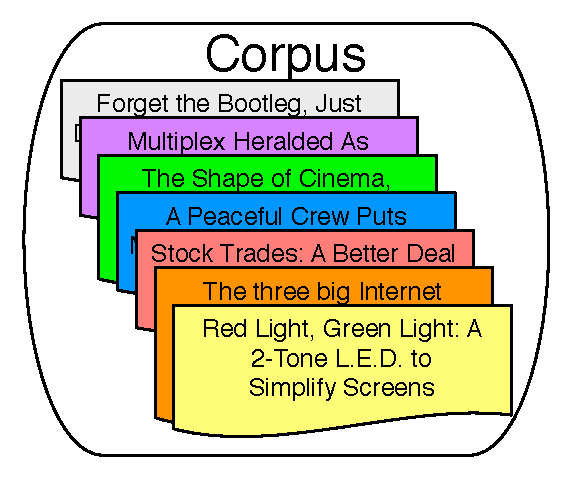
\includegraphics[width=0.6\linewidth]{reading_tea_leaves/figures/heldout_0} }
\only<2>{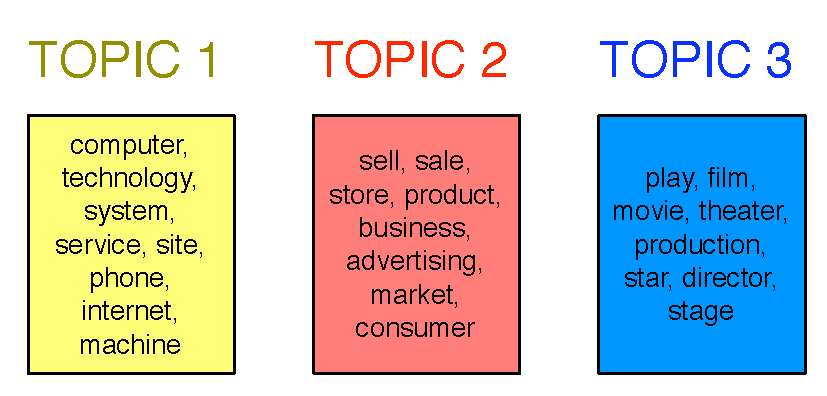
\includegraphics[width=0.9\linewidth]{reading_tea_leaves/figures/nyt_topics_wide}}
%\only<3>{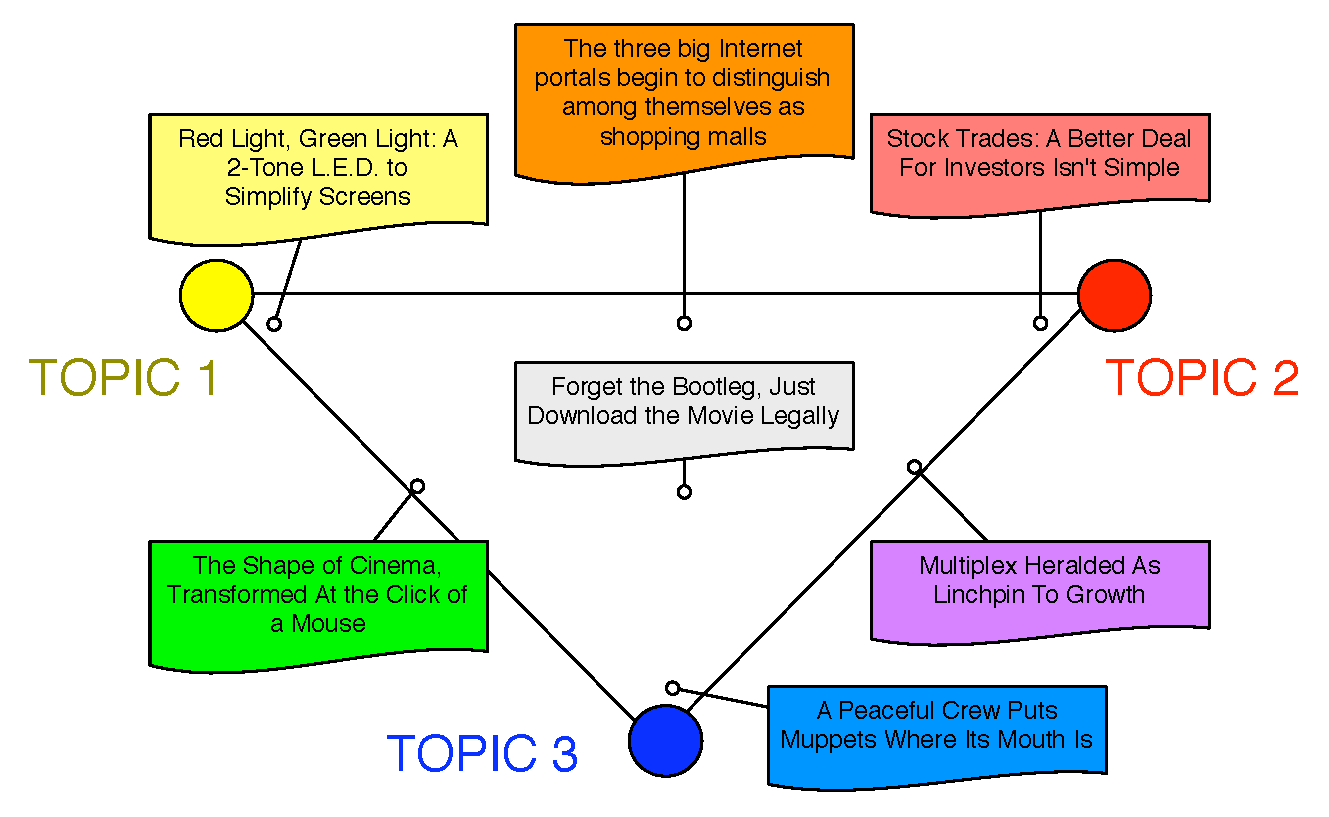
\includegraphics[width=0.9\linewidth]{topic_models/nyt_documents}}
\end{center}

\end{frame}


\begin{frame}{Evaluating Topic Models}

\begin{columns}

\column{.6\linewidth}
\begin{block}{ Reading Tea Leaves: How Humans Interpret Topic Models}
Jonathan Chang, Jordan Boyd-Graber, Chong Wang, Sean Gerrish, and David
M. Blei. Reading Tea Leaves: How Humans Interpret Topic Models. Neural
Information Processing Systems, 2009.
\end{block}

\column{.3\linewidth}
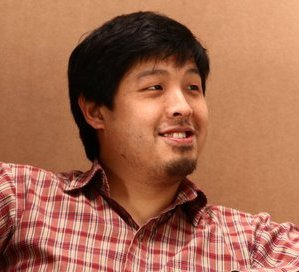
\includegraphics[width=.8\linewidth]{general_figures/jonathan}

\end{columns}

\end{frame}



\frame{
\frametitle{Evaluation}
\begin{center}
%\only<1>{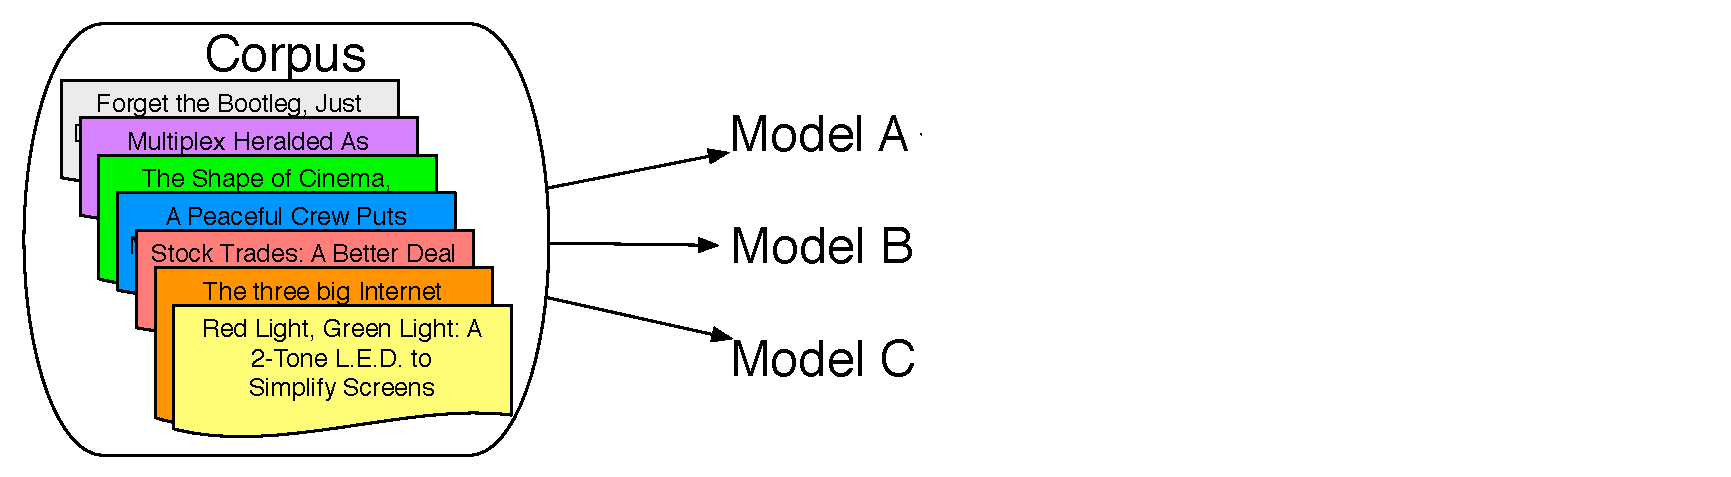
\includegraphics[width=0.9\linewidth]{reading_tea_leaves/figures/heldout_1} }
\only<1>{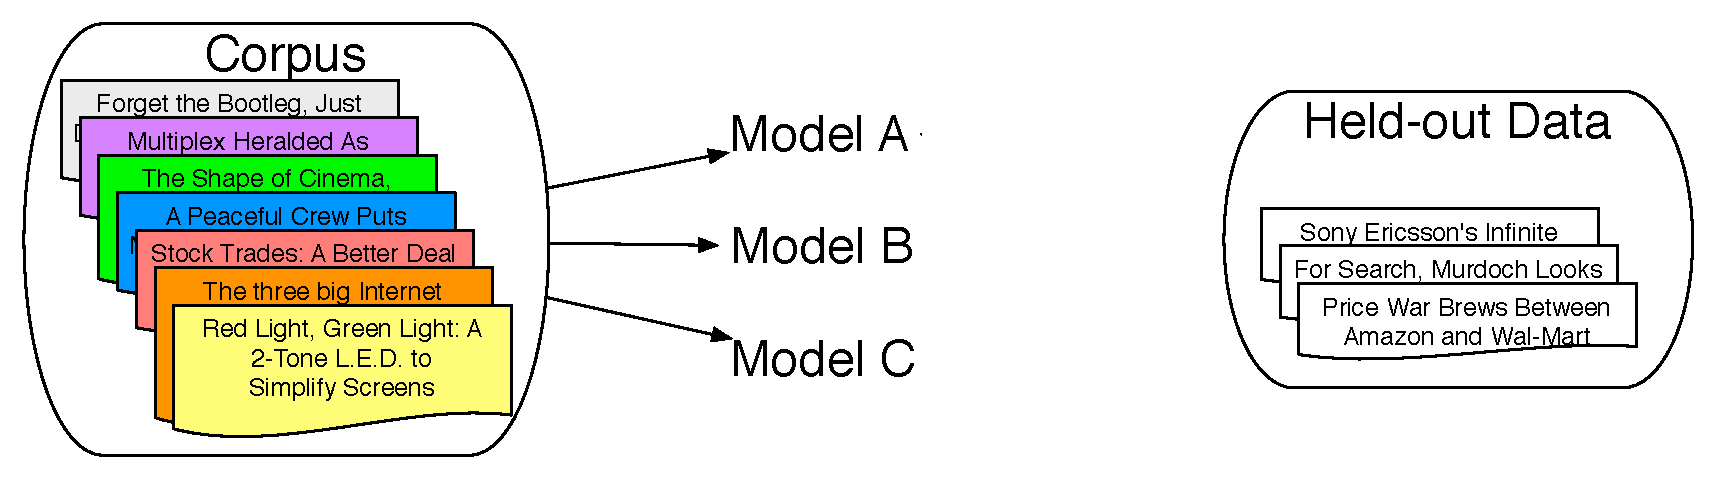
\includegraphics[width=\linewidth]{reading_tea_leaves/figures/heldout_2} }
%\only<3>{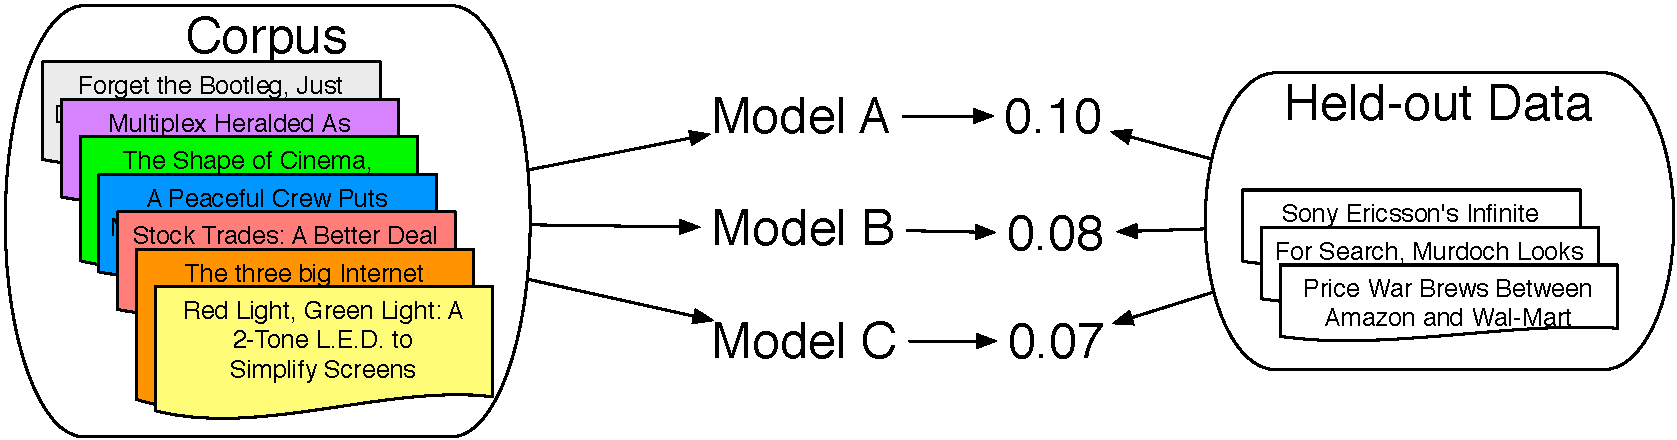
\includegraphics[width=\linewidth]{reading_tea_leaves/figures/heldout_3} }
\only<2>{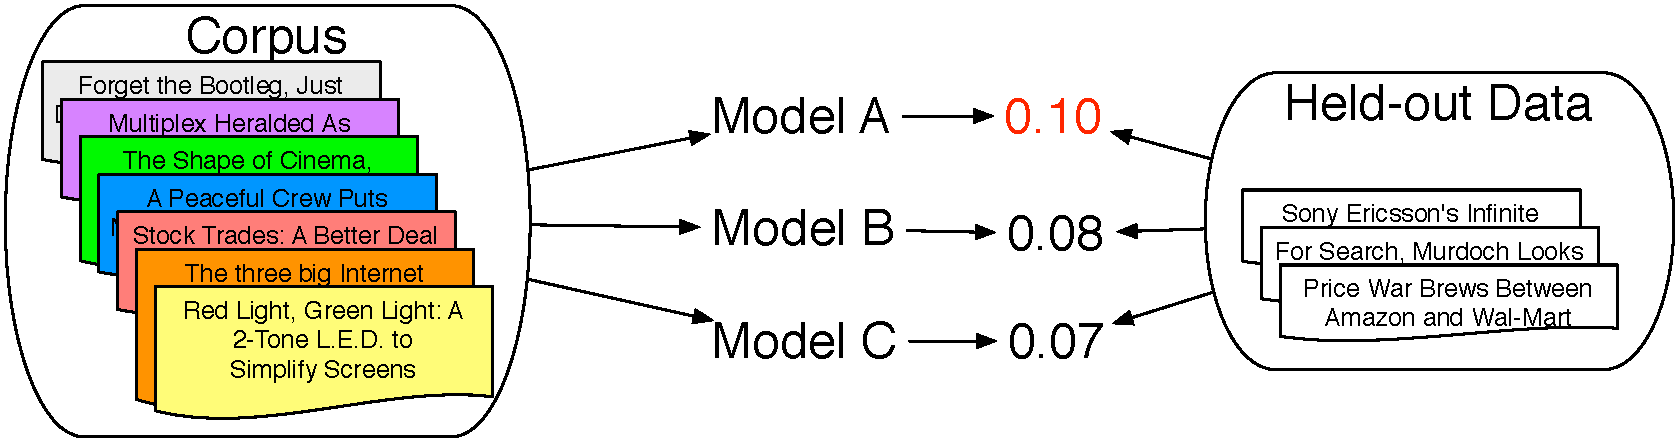
\includegraphics[width=\linewidth]{reading_tea_leaves/figures/heldout_4}  \\
	\large Measures predictive power (likelihood)}
\end{center}
}

\frame{
  \frametitle{Word Intrusion}

  \begin{itemize}
    \item Take the highest probability words from a topic

      \begin{block}{Original Topic}
        dog \\ cat \\ \only<2->{\alert<2->{apple} \\ } horse \\ pig \\ cow
      \end{block}

\only<2->{    \item \alert<2>{Intruder: high probability word from another topic}}
\pause
  \end{itemize}
}

\frame{
\frametitle{Interpretability and Likelihood}


\begin{center}
\only<1>{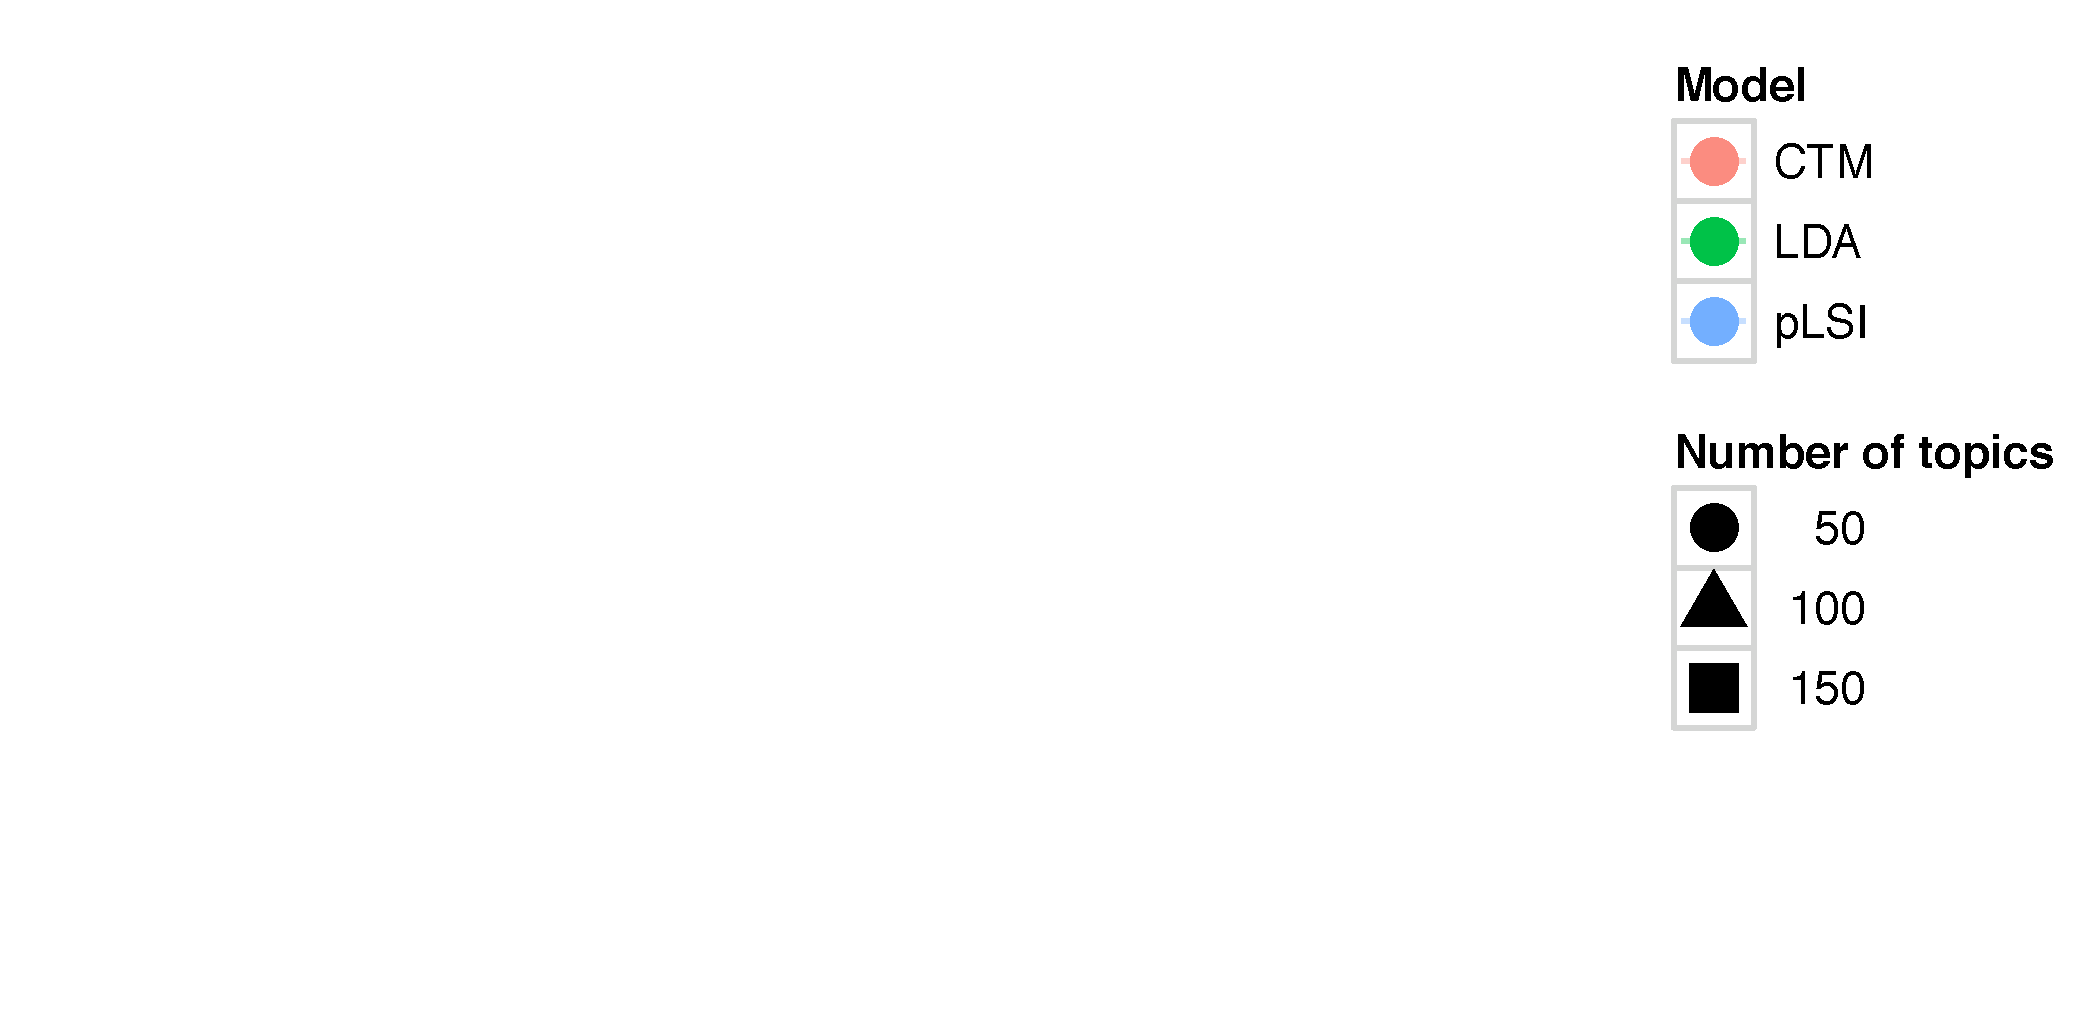
\includegraphics[width=.8\paperwidth]{reading_tea_leaves/figures/prec_ll_1}}
\only<2>{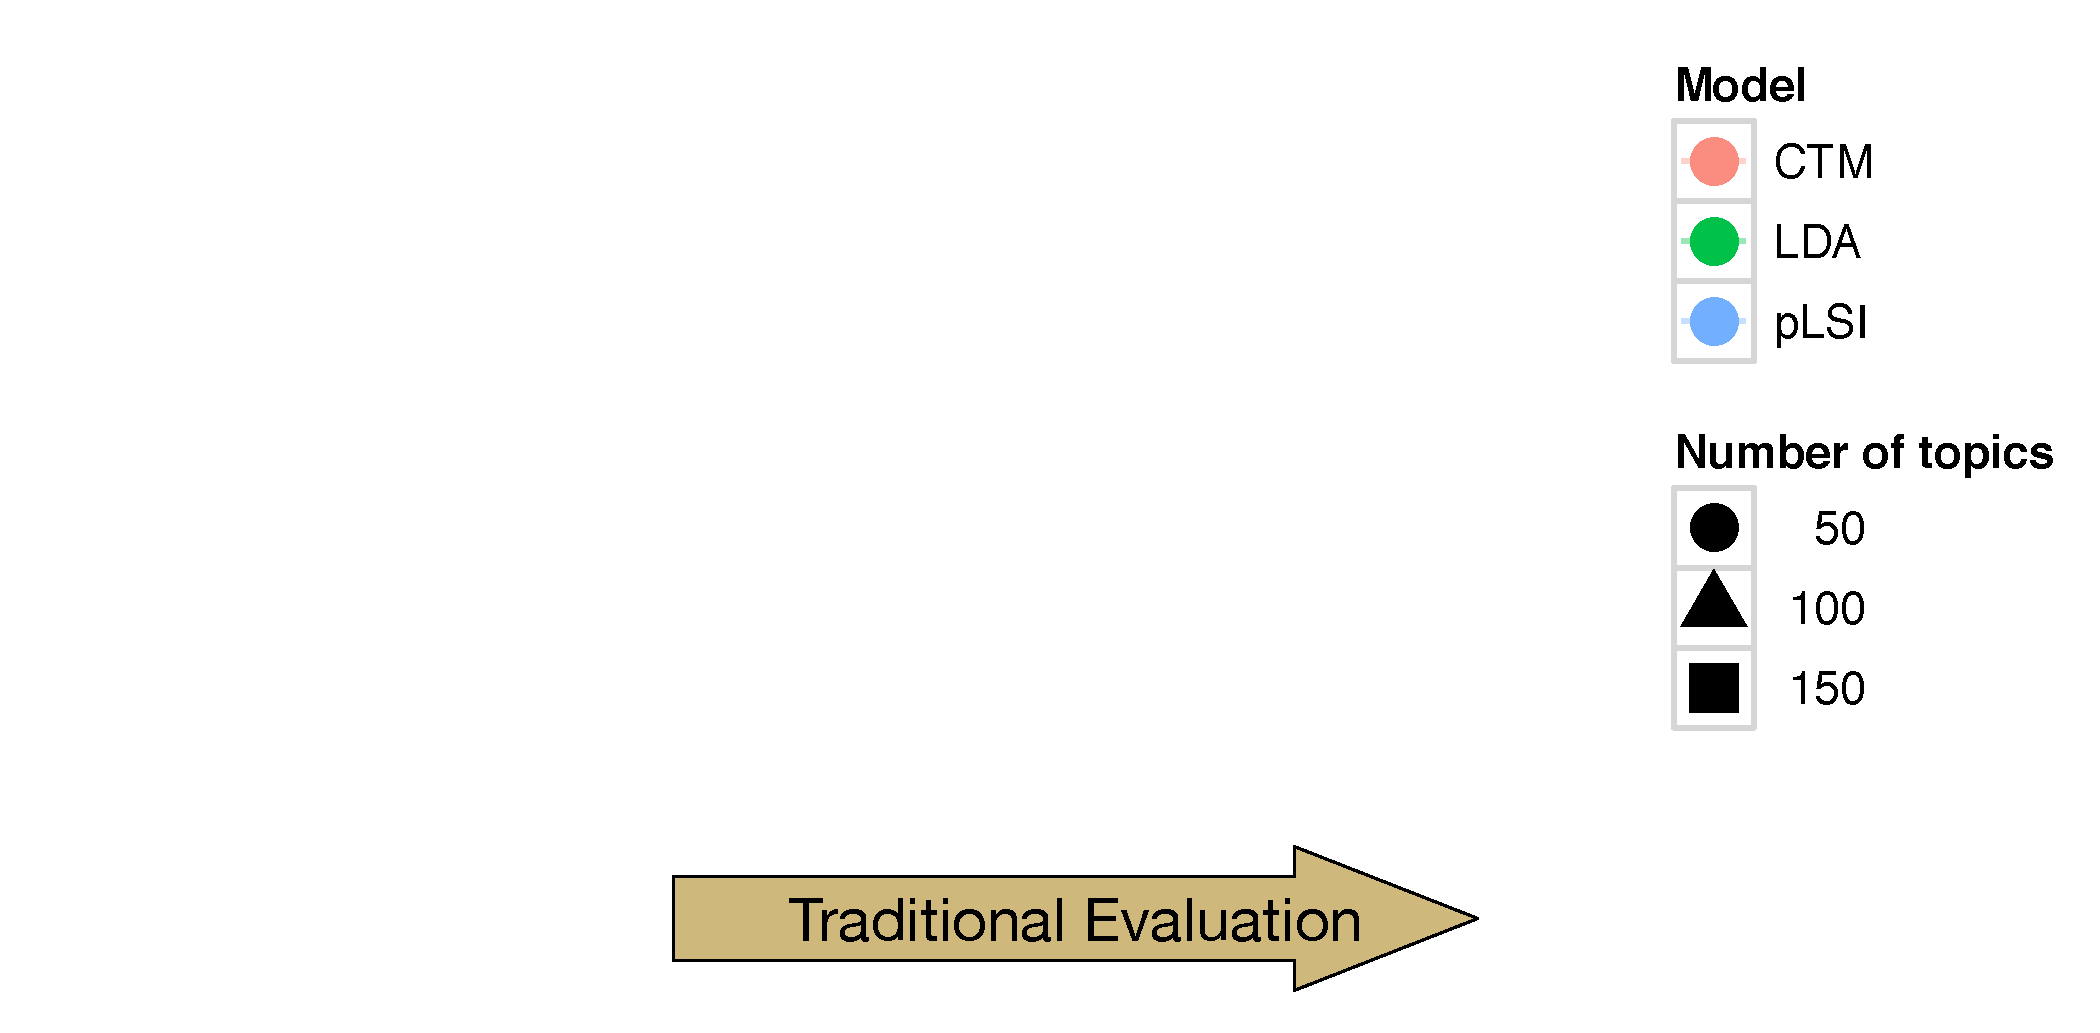
\includegraphics[width=.8\paperwidth]{reading_tea_leaves/figures/prec_ll_2}}
\only<3>{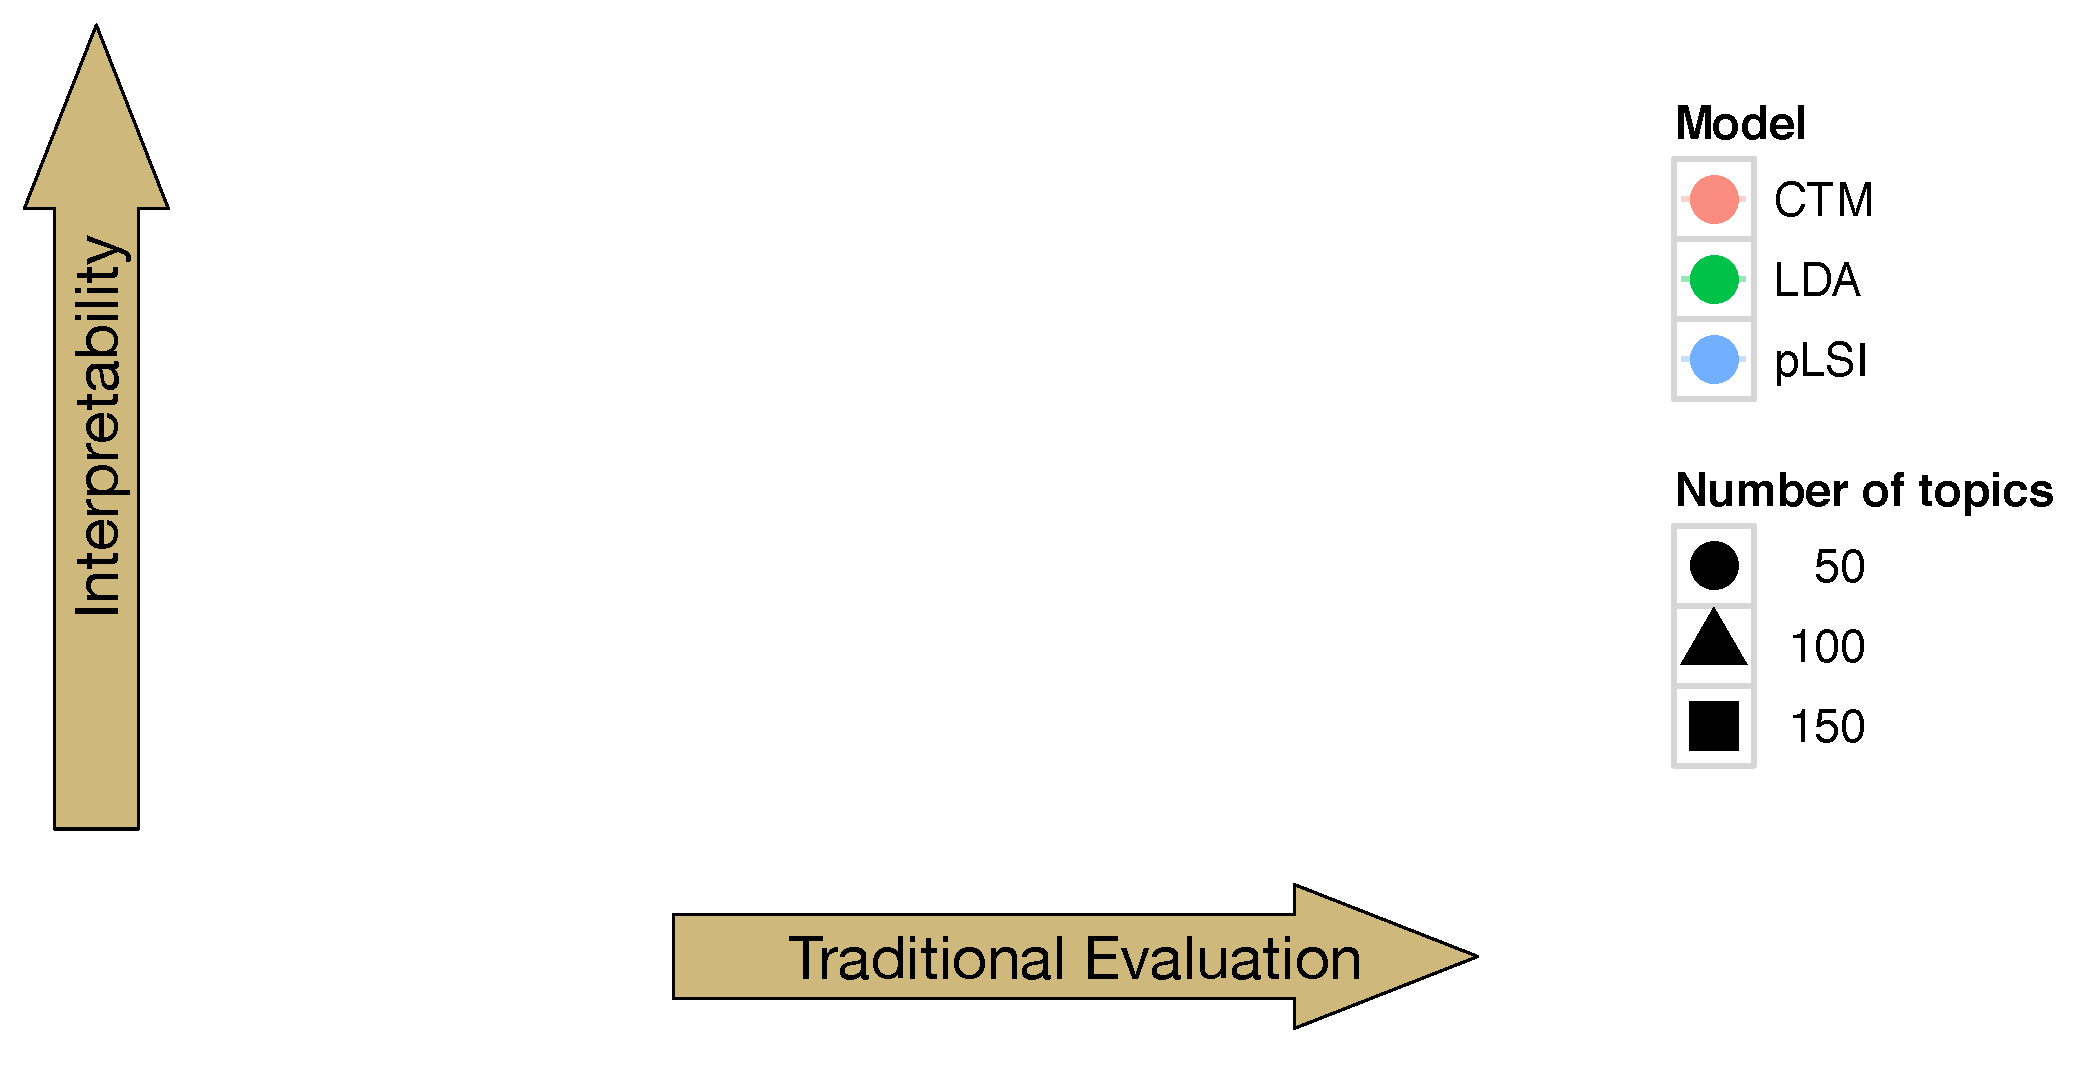
\includegraphics[width=.8\paperwidth]{reading_tea_leaves/figures/prec_ll_3}}
\only<4>{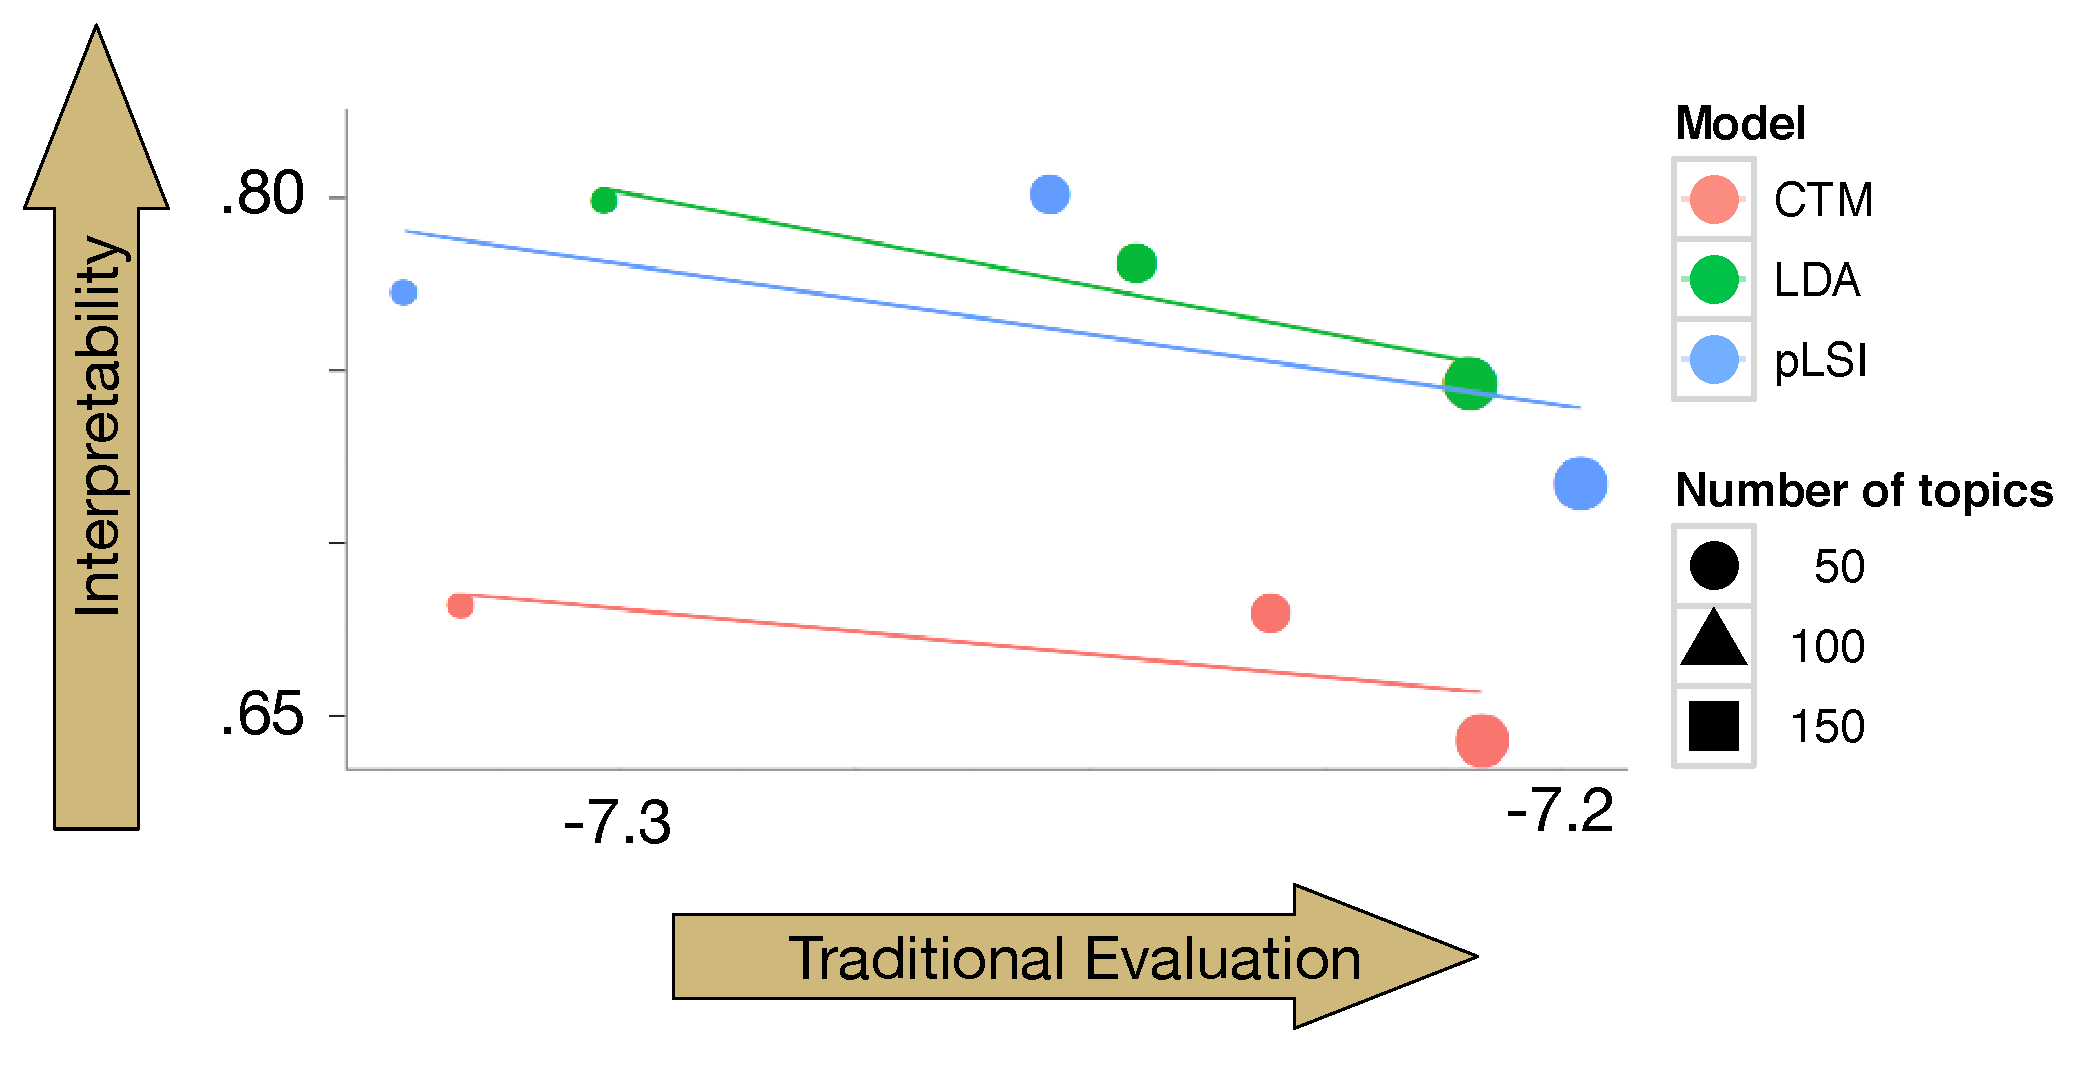
\includegraphics[width=.8\paperwidth]{reading_tea_leaves/figures/prec_ll_4}}
\only<4>{\\ Within a model, higher likelihood $\not =$ higher interpretability}
\end{center}
}





\begin{frame}
\frametitle{The Problem: User Perspective}

\begin{columns}

\column{.4\linewidth}
\begin{center}
\begin{tabular}{ccc}
& \only<2->{\itmspace}\color<2->{red}{bladder} & \\
& \only<3->{\hspace{-2cm}} \color<3->{blue}{spinal\_cord}  & \\
& \only<3->{\hspace{-2cm}} \color<3->{blue}{sci} & \\
& \only<3->{\hspace{-2cm}}\color<3->{blue}{spinal\_cord\_injury} & \\
& \only<3->{\hspace{-2cm}}\color<3->{blue}{spinal} & \\
& \only<2->{\itmspace}\color<2->{red}{urinary} & \\
& \only<2->{\itmspace}\color<2->{red}{urothelial} & \\
& \only<3->{\hspace{-2cm}}\color<3->{blue}{cervical} & \\
& injury & \\
& recovery & \\
& \only<2->{\itmspace}\color<2->{red}{urinary\_tract} & \\
& locomotor & \\
& \only<3->{\hspace{-2cm}}\color<3->{blue}{lumbar} & \\
\end{tabular}
\end{center}

\column{.6\linewidth}

\danquote{These words don't belong together!}

\end{columns}

\end{frame}


\frame{

\begin{columns}

\column{.5\linewidth}

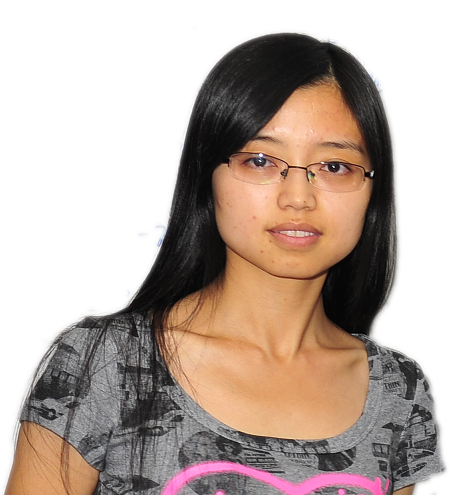
\includegraphics[width=.8\linewidth]{general_figures/yuening}

\column{.5\linewidth}

\begin{block}{Interactive Topic Modeling}
Yuening Hu, Jordan Boyd-Graber, and Brianna Satinoff.  Association for Computational Linguistics, 2011.
\end{block}


\end{columns}

}



\frame{
	\frametitle{How to fix it?}


	\only<1>{	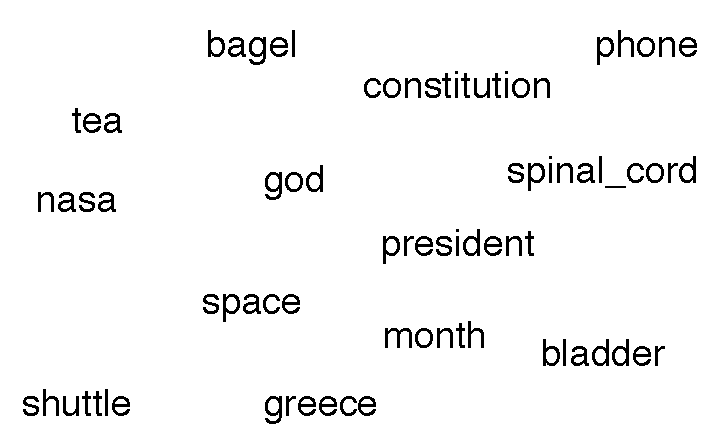
\includegraphics[width=\linewidth]{interactive_topic_models/constraints_1}     }
	\only<2>{	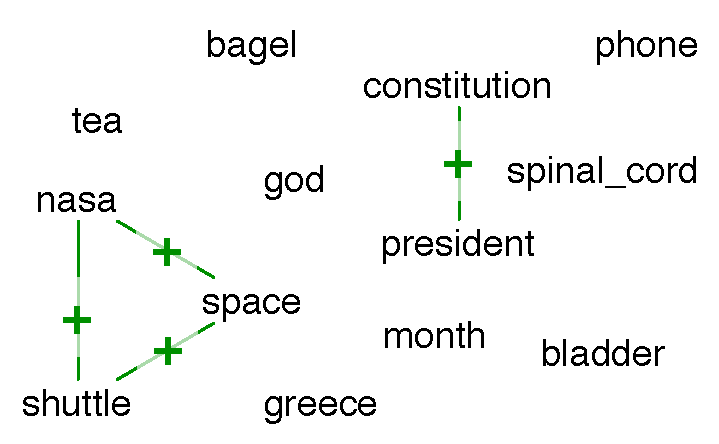
\includegraphics[width=\linewidth]{interactive_topic_models/constraints_2}     }
	\only<3>{	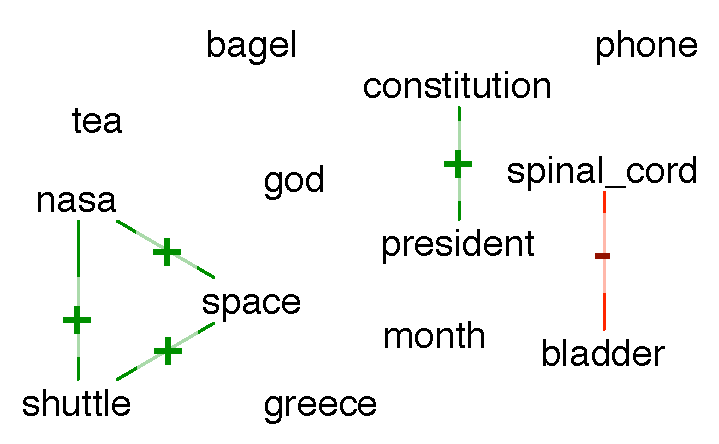
\includegraphics[width=\linewidth]{interactive_topic_models/constraints_3}     }


}


\providecommand{\tb}[1]{\parbox{0.8\linewidth}{ \tiny{ #1 }} \vspace{.2cm} }

\frame{

\vspace{-1cm}

\begin{columns}

\column{.5\linewidth}

\begin{tabular}{l*{2}{c}r}
	Topic & Before \\
\hline

\alert<2>{{\bf 1}} & \tb{ \alert<2>{election, yeltsin, russian, political, party, democratic, russia,
  president, democracy, boris, country, south, years, month, government, vote,
  since, leader, presidential, military} } \\

2 & \tb{new, york, city, state, mayor, budget, giuliani, council, cuomo, gov,
  plan, year, rudolph, dinkins, lead, need, governor, legislature, pataki,
  david} \\

3 & \tb{nuclear, arms, weapon, defense, treaty, missile, world, unite, yet,
  soviet, lead, secretary, would, control, korea, intelligence, test, nation,
  country, testing} \\

4 & \tb{president, bush, administration, clinton, american, force, reagan, war,
  unite, lead, economic, iraq, congress, america, iraqi, policy, aid,
  international, military, see} \\

& \vdots \\

\alert<2>{{\bf 20}} & \tb{\alert<2>{soviet, lead, gorbachev, union, west, mikhail, reform, change, europe,
  leaders, poland, communist, know, old, right, human, washington, western,
  bring, party} }\\

\end{tabular}

\column{.5\linewidth}

\only<3> {

	\begin{block}{Suggestion}
	\emph{boris, communist, gorbachev, mikhail, russia,
  russian, soviet, union, yeltsin }
	\end{block}

}

\only<4-> {

\begin{tabular}{l*{2}{c}r}
	Topic & After \\
\hline

\alert<5>{{\bf 1}} & \alert<5>{\tb{election, democratic, south, country, president, party, africa, lead,
  even, democracy, leader, presidential, week, politics, minister, percent,
  voter, last, month, years} } \\

\alert<6>{2} & \tb{new, york, city, state, mayor, budget, council, giuliani, gov, cuomo,
  year, rudolph, dinkins, legislature, plan, david, governor, pataki, need, cut}
\\

\alert<6>{3} & \tb{nuclear, arms, weapon, treaty, defense, war, missile, may, come, test,
  american, world, would, need, lead, get, join, yet, clinton, nation} \\

\alert<6>{4} & \tb{president, administration, bush, clinton, war, unite, force, reagan,
  american, america, make, nation, military, iraq, iraqi, troops, international,
  country, yesterday, plan} \\

   & \vdots \\

\alert<4>{ {\bf 20} } & \alert<4> {\tb{soviet, union, economic, reform, yeltsin, russian, lead, russia,
  gorbachev, leaders, west, president, boris, moscow, europe, poland, mikhail,
  communist, power, relations} } \\

\end{tabular}

}

\end{columns}

}


\providecommand{\blue}[1]{{\color{blue}{#1}}}
\providecommand{\red}[1]{{\color{red}{#1}}}
\providecommand{\green}[1]{{\color{green}{#1}}}

\begin{frame}

\frametitle{Example: Negative Constraint}

\begin{columns}

\column{.4\linewidth}

\begin{tabular}{l*{2}{c}r}
	Topic & Words \\
\hline

{\bf 318} & \tb{\red{bladder}, sci, \blue{spinal\_cord}, \blue{spinal\_cord\_injury}, \blue{spinal}, \red{urinary}, \red{urinary\_tract}, \red{urothelial},\blue{injury}, \blue{motor}, \blue{recovery}, \blue{reflex}, \blue{cervical}, \red{urothelium}, \blue{functional\_recovery}} \\

\end{tabular}

\column{.1\linewidth}

\column{.4\linewidth}

\only<3->{
\begin{tabular}{l*{2}{c}r}
	Topic & Words \\
\hline

{\bf 318} & \tb{sci, \blue{spinal\_cord}, \blue{spinal\_cord\_injury}, \blue{spinal}, \blue{injury}, \blue{recovery}, \blue{motor}, \blue{reflex}, \red{urothelial}, \green{injured}, \blue{functional\_recovery}, \green{plasticity}, \green{locomotor}, \blue{cervical}, \green{locomotion}}\\

\end{tabular}
}

\end{columns}

\only<2->{
\begin{block}{Negative Constraint}
  spinal\_cord, bladder
\end{block}

}

\end{frame}



\begin{frame}{Representing Elected Officials: Ideal Points}
  \gfxt{dw_nominate}{.7}

  An essential tool in political science: distinguish trends and characterize subgroups
\end{frame}

\fsi{qb/karl}{http://karl.qanta.org}


\fsi{qb/augment/screenshot_all}{Interface}

\fsi{qb/augment/screenshot_guesses}{}

\fsi{qb/augment/screenshot_highlight}{{\bf Highlighting}}

\fsi{qb/augment/screenshot_evidence}{}

\begin{frame}{Experts vs. Novices}

 \begin{block}{Experts}
   Trivia experts, familiar with task, enjoy the task
 \end{block}

 \begin{block}{Mechanical Turkers}
   Mechanical Turkers: easily overwhelmed, need the help
 \end{block}

\end{frame}

\fsi{qb/augment/tools_acc}{Evidence helps novices, experts are expert}
\fsi{qb/augment/tools_buzz}{Hights help experts}



\fsi{qb/human_reading}{SQuAD: Ignore Knowledge}

\fsi{qb/jeopardy}{IBM Watson: QA Solved!}


\begin{frame}{Ambiguous Questions}
  \rowcolors{2}{gray!25}{white}
  \begin{small}
  \begin{tabular}{p{7cm}p{3cm}}
    \toprule
    Question & Gold Answer \\
    \hline
    \alert<2>{when was the last time michigan won the championship} & 1989 \\
    \alert<3>{what year did the us hockey team won the olympics} & 1960 and 1980 \\
    \alert<4>{which supreme court judge has surved in international court of justice} & Dalveer Bhandari \\
    \alert<5>{where does puerto rico's power come from} & Puerto Rico Electric Power Authority \\
    \bottomrule
  \end{tabular}
  \end{small}
  \begin{block}{Assumptions\dots}
  \only<2>{NCAA Division I Men's Football}
  \only<3>{Men's competition}
  \only<4>{Indian Supreme Court}
  \only<5>{Electric power}
  \only<6>{Bias for Men's sports, especially football.  Ambiguity is arbitrarily resolved by search engine result.}
  \end{block}
\end{frame}




\begin{frame}{Representation in QA}

    \resizebox{.75\linewidth}{!}{%
        \begin{tabular}{c l rr rr rr rr}
        % \hline
        % \multicolumn{2}{c}{\small{\textbf{Demography}}}  & \textbf{\nq} & \textbf{\qb} & \textbf{\squad} & \textbf{\triviaqa} \\
        \hspace{15pt} & \multirow{2}{*}{\textbf{Value}} %{\small{\textbf{Value}}}  
            & \multicolumn{2}{c}{\textbf{\nq}} 
            & \multicolumn{2}{c}{\textbf{\qb}}  
            & \multicolumn{2}{c}{\textbf{\squad}}  
            & \multicolumn{2}{c}{\textbf{\triviaqa}} \\ 
        
        & 
            & \hspace{5pt}\textbf{Train} & \textbf{Dev} 
            & \hspace{5pt}\textbf{Train} & \textbf{Dev} 
            & \hspace{5pt}\textbf{Train} & \textbf{Dev} 
            & \hspace{5pt}\textbf{Train} & \textbf{Dev}\\ 
        
        \toprule
        \multirow{3}{*}{\rotatebox[origin=c]{90}{\textbf{Gender}}}
            & Male    
                &  \textbf{75.67} &  \textbf{76.33} 
                &  \textbf{91.77} &  \textbf{91.63} 
                &  \textbf{87.82} &  \textbf{95.15} 
                &  \textbf{83.76} &  \textbf{83.32} \\
               
            & Female          
                &  27.47 &  27.56 
                &  10.29 &   9.87 
                &  13.44 &   5.20 
                &  20.54 &  20.29 \\
                
                % &   0.31 &   0.35 &   0.27 &   0.30
            % & Other           &   0.12 &   0.00 &   0.09 &   0.12 \\
            & No Gender
                &   0.31  &   0.47
        		&   0.35  &   0.39
        		&   0.27  &   0.00
        		&   0.30  &   0.35 \\
        \midrule
        \multirow{3}{*}{\rotatebox[origin=c]{90}{\textbf{Country}}}
            & US
                & \textbf{59.62}	& \textbf{58.66}
        		& \textbf{29.70}	& \textbf{26.28}
        		& \textbf{32.74}	& \textbf{24.93}
        		& 31.32	& 30.91
                \\
            
            & UK
        		& 15.76	& 15.78
        		& 17.92	& 17.68
        		& 19.66	& 16.83
        		& \textbf{41.92}	& \textbf{41.32}
        		\\
            
            & France
        		& 1.79	& 1.18
        		& 10.06	& 10.34
        		& 7.76	& 10.57
        		& 4.37	& 4.84
        		\\
            

        \midrule
        \multirow{4}{*}{\rotatebox[origin=c]{90}{\textbf{Field}}}
            & Film/TV
				& \textbf{39.19}	& \textbf{37.93}
				& 3.16	& 1.89
				& 10.72	& 1.32
				& 20.64	& \textbf{20.75}
				\\
            
            & Writing 
				& 7.40	& 6.95
				& \textbf{36.62}	& \textbf{36.39}
				& 10.46	& 6.70
				& 18.41	& 18.05
				\\
				
            & Politics 
				& 11.98	& 10.84
				& 24.02	& 24.86
				& \textbf{36.97}	& \textbf{46.61}
				& \textbf{21.18}	& 20.72
				\\
				
            & Science/Tech
				& 3.61	& 4.71
				& 8.93	& 7.50
				& 13.67	& 29.60
				& 5.43	& 5.54
				\\
				
				
\bottomrule \end{tabular}}

\end{frame}

\begin{frame}{QA in low resource languages: Adaptation}

  \begin{tabular}{p{3cm} p{6cm}}
	\label{tab:de_veale_human}
	\bf Entity & \bf Human Adaptation \\
	\toprule
	%\noalign{\vskip 2mm} 
Otto von Bismarck & George Washington,	George Washington,	Ulysses S. Grant,	George Washington,	George Washington,	Abraham Lincoln \\
Martin Luther & Brigham Young,	Joseph Smith,	Barry Goldwater,	Joseph Smith,	Joseph Smith\\
Karl Lagerfeld & Anna Wintour,	Ralph Lauren,	Anna Wintour,	Ralph Lauren,	Ralph Lauren,	Marc Jacobs,	Ralph Lauren \\
Angela Merkel & Hillary Clinton,	Hillary Clinton,	Donald Trump,	Joe Biden,	Hillary Clinton,	Barack Obama,	Hillary Clinton \\
Immanuel Kant & Benjamin Franklin,	John Dewey,	John Rawls,	John Locke,	Robert Nozick \\
Richard Wagner &	Charles Ives,	Frank Sinatra,	Leonard Bernstein,	Philip Glass \\
    Carl von Clausewitz & Robert E. Lee,	Alfred Thayer Mahan,	Dwight D. Eisenhower,	Ulysses S. Grant,	Henry Knox \\
    \bottomrule
    \end{tabular}
  \end{frame}




\begin{frame}{Trick me if you can\dots}

  \begin{itemize}
  \item Trivia writers create questions
  \item {\bf Current} explain why they answer (and when)
  \item Trivia writers make questions go from hard to easy (for both
    humans and computers)
    \pause
    \item \only<2>{PROFIT!} \only<3>{Better questions!}
  \end{itemize}

\end{frame}

% \begin{frame}{What do we mean by ``adversarial''?}

%   \gfxq{trick/flow_chart_horizontal_label}{1.0}

%   \begin{itemize}
%     \item Both neural and IR systems
%       \pause
%     \item Reason we need to have good explanations of QA
%   \end{itemize}

% \end{frame}

\fsi{qb/trick/brahms_0}{\href{http://write.qanta.org}{http://write.qanta.org}}
\fsi{qb/trick/brahms_1}{}
\fsi{qb/trick/brahms_2}{}
\fsi{qb/trick/brahms_3}{}
\fsi{qb/trick/brahms_4}{}
\fsi{qb/trick/brahms_5}{}


\fsi{qb/trick/round_one}{Just as easy for humans, harder for computers.}




\begin{frame}{Linguistics FTW}

  The main character of a story by \alert<2>{this author opens Crime and Punishment} to a
random page, but finds it to be a copy of The Brother Karamazov, and equates
himself with Monsieur Bovary. This author wrote a story in which the priest
Naigu undergoes a boiling treatment to decrease the size of his nose. This
author of "Cogwheels" wrote about two people who steal to survive near the
southern gate of Kyoto in a story that features inconsistent accounts from a
woodcutter, a priest, a widow, and the ghost of a samurai. For 10 points, name
this author of "Rashomon" and namesake of a Japanese literary prize. \\
\only<3->{\textbf{Answer}: Ryunosuke Akutagawa}
\end{frame}


\fsi{qb/jennings_handshake}{}

\begin{frame}[plain]
\gfxq{seattle_crowd}{.5}
\gfxq{chicago_crowd}{.5}
\end{frame}



\frame{
  \frametitle{But wait, there's more!}

  \vspace{-.5cm}

\begin{columns}



  \column{.5\linewidth}

   \begin{block}{Computational Biology}
     \centering
     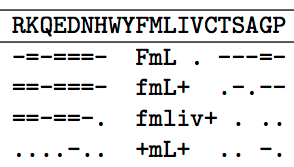
\includegraphics[width=0.4\linewidth]{general_figures/protein} \\
     \small
     \cite{nguyen-13b,hu-13:coalescent}
   \end{block}



    \begin{block}{Interactive Machine Learning}
     \centering
        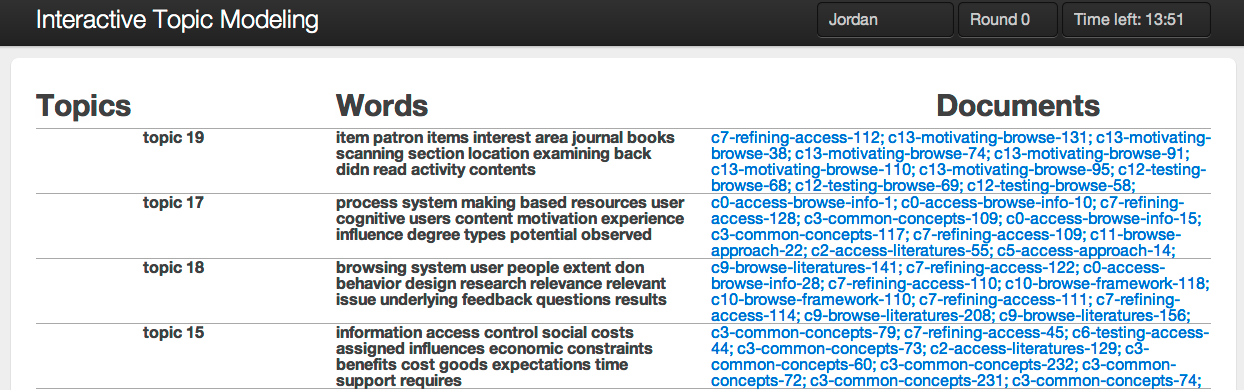
\includegraphics[width=0.4\linewidth]{interactive_topic_models/new_interface} \\
       \cite{Smith-17,Poursabzi-16}
    \end{block}


  \column{.5\linewidth}


    \begin{block}{Multilingual Analysis / Machine Translation}
      \begin{center}
        \begin{large}
          $p_{\mbox{topic}}(e | f)$ \\
         \end{large}
      \cite{eidelman-12,hu-14}
       \end{center}
    \vspace{-.3cm}
    \end{block}


    \begin{block}{Detecting Deception}
    \centering
        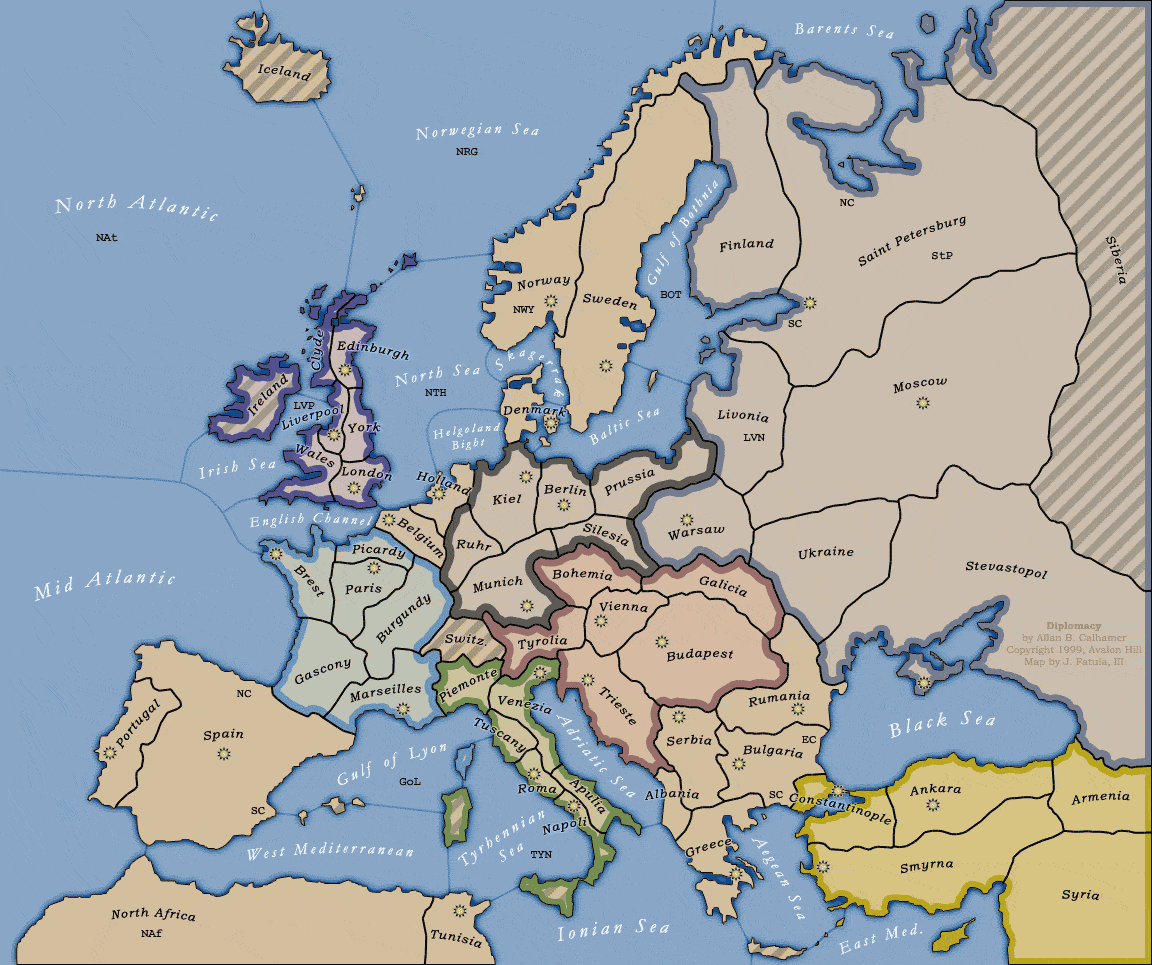
\includegraphics[width=0.4\linewidth]{general_figures/diplomacy} \\
        \cite{niculae-15,peskov-20}
    \end{block}




\end{columns}

}

\begin{frame}{Sabotaged by IR}

  \rowcolors{2}{gray!25}{white}
  \begin{small}
  \begin{tabular}{p{7cm}p{3cm}}
    \toprule
    Question & Page \\
    \hline
 when did the states secede during the civil war &  Border states (American Civil War) \\
 who wears number 2 for the dallas cowboys &  Jeff Heath (American football) \\
 how many countries participated for the first time in the 2014 olympic winter games in sochi & 2014 Winter Paralympics \\
 game of thrones season 7 number of episoded &  List of Teen Wolf episodes \\
 \bottomrule
  \end{tabular}
  \end{small}

\end{frame}

\begin{frame}{Good for Search, Bad for QA}

  Title of page is answer, annotators didn't find span:
  \rowcolors{2}{gray!25}{white}
  \begin{tabular}{p{7cm}p{3cm}}
    \toprule
    Question & Page \\
    \hline
  who plays the goblin king in the hobbit &  Barry Humphries  \\
  who does the voice of fart in rick and morty & Jemaine Clement   \\
 \bottomrule
  \end{tabular}
\end{frame}

\begin{frame}{Questions Depends on Who / When}
  \rowcolors{2}{gray!25}{white}
  \begin{tabular}{p{8cm}p{2cm}}
    \toprule
    Question & Gold Answer \\
    \hline
    can i buy wine in kentucky on sunday & --- \\
    where am i on the steelers waiting list & --- \\
    when is the real housewives on & --- \\
    who has majority in the house and senate & --- \\
    \bottomrule
  \end{tabular}  

  \pause

  \begin{block}{Answerable Questions\dots}
  But depend on which county of Kentucky you're in,
  when you paid for your season pass, and the local network
  syndicating Real Housewives.
  \end{block}
  
\end{frame}


\begin{frame}{References}
\bibliographystyle{style/acl}
\tiny
\bibliography{bib/journal-full,bib/jbg}
\end{frame}



\end{document}